\documentclass[a4paper]{scrartcl}
%to print this use ,twoside

\usepackage[automark,headsepline,footsepline]{scrlayer-scrpage}
\usepackage{lmodern}
\usepackage[ngerman]{babel}
\usepackage[T1]{fontenc}
\usepackage[utf8]{inputenc}
\usepackage{framed}
\usepackage{setspace}
\usepackage{lastpage}
\usepackage{amssymb}
\usepackage[intlimits]{amsmath}
\usepackage{amstext}
\usepackage{amsfonts}
\usepackage{mathrsfs}
\usepackage [pdftex]{graphicx}
\usepackage{tcolorbox}
\usepackage{color}

\usepackage{graphics}
\usepackage{svg}
\usepackage{tikz}

\usepackage{tabularx}


% set colors for links and URLs
\usepackage[
colorlinks=true,
urlcolor=blue,
linkcolor=black
]{hyperref}


\setlength{\parindent}{0pt} %remove awful indent from new paragraphs

%color definitions
\definecolor{navyblue}{cmyk}{1, 1, 0, 0.5}
\definecolor{lightorange}{cmyk}{0,0.5,1,0}
\definecolor{lightgrey}{cmyk}{0,0,0,0.1}
\definecolor{mediumgrey}{cmyk}{0,0,0,0.4}
\definecolor{whitegrey}{cmyk}{0,0,0,0.02}
\definecolor{drkred}{cmyk}{0,1,1,0}
\definecolor{darkred}{cmyk}{0,1,1,0.25}


%definitions for the title page
\def \mTitle {SoPlan}
\def \mLongTitle{SoPlan\\Studienprojekt}
\def \mSubtitle {Entwicklung eines IT-gestützten Verwaltungstools für Schülerakademien.}
\def \mAuthor {}
\def \mPublisher {Projektplan Studienprojekt}
\def \mDate {14. Oktober 2018}

\newcommand{\mTitlePage}[0]
{
	\begin{titlepage}
		\begin{flushleft}
			\textsf{
				\hrule
				\vspace{0.5cm}
				\LARGE \mAuthor \hfill \mDate \\
				\vspace{0.5 cm}
				{\fontsize{100}{60} \selectfont \mTitle} \\
				\vspace{0.5cm}
				\Large \mSubtitle \\
				\vspace{0.5cm}
				\hrule
				\vspace{2.5cm}
				\centering{
\includegraphics[width=400pt,keepaspectratio]{Logo_RUB_BLAU_cmyk.jpg}}
				\vfill
				\LARGE \mPublisher \\
				\normalsize
			}
		\end{flushleft}
	\end{titlepage}
	\pagebreak \eject
}

\newcommand{\mybox}[1]{%
	\setbox0=\hbox{#1}%
	\setlength{\@tempdima}{\dimexpr\wd0+13pt}%
	\begin{tcolorbox}[colframe=mycolor,boxrule=0.5pt,arc=4pt,
		left=6pt,right=6pt,top=6pt,bottom=6pt,boxsep=0pt,width=\@tempdima]
		#1
	\end{tcolorbox}
}

\newcommand\mTab[1][1cm]{\hspace*{#1}}

\pagestyle{scrheadings}

\clearscrheadfoot

\setkomafont{pageheadfoot}{\upshape}
\setkomafont{pagehead}{\upshape}
\setkomafont{headsepline}{\color{mediumgrey}}
\setkomafont{footsepline}{\color{mediumgrey}}

\ohead[]{
\includegraphics[height=1cm]{Logo_RUB_BLAU_cmyk.jpg}}
\ihead[]{\textsf{\mLongTitle}}

\addtokomafont{pagenumber}{\sffamily}
\ofoot{\textsf{Seite \pagemark\ von \pageref{LastPage}}}

\begin{document}
	
\mTitlePage
	
\section*{Hinweis}
	In diesem Dokument wird an den meisten Stellen die männliche Wortform genutzt, um die Lesbarkeit zu wahren. An jeder Stelle ist ebenso selbstverständlich die weibliche Wortform mit eingeschlossen.
	\\
	
	\vfill
	
	\begin{tcolorbox}[colframe=navyblue,colback=whitegrey,boxrule=0.5pt,arc=2pt,
		left=8pt,right=8pt,top=8pt,bottom=8pt,boxsep=0pt,width=\textwidth]
		\LARGE{SoPlan}\normalsize\\\\
		Der Name \emph{SoPlan} ist der Arbeitstitel dieses Projekts. Ein geeigneter Produktname muss im Projektverlauf festgelegt werden.
	\end{tcolorbox}

\pagebreak
\eject

\tableofcontents

%\vfill


\pagebreak
\eject

\section*{Projektdaten}
	
	\begin{tabularx}{\textwidth}{|l|X|}
		\hline
		Projektname & SoPlan \\ \hline
		Projektbetreuer & Marcel Schmittchen \& Jonas Herbert \\ \hline
		Auftraggeber & Landesverband Mathematikwettbewerbe NRW e.V.\\ \hline
		Projektstart & 18. August 2018 \\ \hline
		Zuletzt geändert & 06. September 2018 \\ \hline
		Version & SoPlan 1.0.2 \\
		\hline
	\end{tabularx}

	\subsection*{Projektdetails}
	
	\begin{tabularx}{\textwidth}{|l|Xr|}
		\hline
		Mitwirkend && Akkiraz, Tolga \\
		&& Beermann, Robin \\
		&& Kosjakov, Anton \\
		&& Sahin, Abdullah \\ \hline
		Projektstart && 18. August 2018 \\ \hline
		Umsetzungsstart && 08. Oktober 2018 \\ \hline
		Umsetzungsende && 08. Februar 2019 \\ \hline
		Abschlussdokumentation && 08. Februar 2019 \\ \hline
		Projektende && unterminiert \\ \hline
	\end{tabularx}

	\vfill
	
	\begin{quote}
		\textsf{Es gibt viel Spielraum nach unten.}
		\flushright{\textsf{\textit{\textbf{Richard Feynman}, 1918-1988, Physiker}}}
	\end{quote}

\pagebreak
\eject

\section{Vorwort}
	Das vorliegende Dokument stellt alle an das System verbindlich gestellten Anforderungen dar. Es dient als Grundlage zur Entwicklung einer Architektur und Implementation für das Projekt. Zur Umsetzungslaufzeit (d.h. im Rahmen des Studienprojekts 2018/19) sollen die \emph{minimalen} Anforderungen umgesetzt werden. Diese umfassen die grundlegende Struktur und die wesentlichen Funktionen des Programms und werden in diesem Dokument vorgestellt. Weiterhin enthält dieses Dokument zusätzliche, zukünftige Erweiterungen für das Programm.
	
	Ergeben sich während der Umsetzungslaufzeit neue Anforderungen, können diese in das Projekt aufgenommen werden. Eine Aufnahme in das ist nicht gleichzusetzen mit der Umsetzung im Rahmen des Studienprojekts, kann jedoch nach Rücksprache mit dem Auftraggeber erfolgen. Sollten im Laufe der Umsetzung Probleme auftreten, die begründbar eine fristgerechte Fertigstellung gefährden, so können diese in Rücksprache mit dem Auftraggeber gegen anderen Anforderungen ausgetauscht werden. Die Entscheidungsgewalt darüber obliegt dem Auftraggeber.
	
\section{Zielbestimmung}
	\subsection{Ausgangslage}
	Der Landesverband Mathematikwettbewerbe NRW e.V. richtet jährlich verschiedene Schülerakademien und Förderungswochenenden aus.
	
	\emph{Arbeitsdefinition}: Eine Schülerakademie ist eine Fortbildungsveranstaltung zur Förderung von begabten Schülern, die über den normalen Unterricht hinausgeht und nicht von einem Schulträger veranstaltet wird.
	
	\subsubsection{Phasen}
	Jede Schülerakademie folgt ungefähr dem gleichen Muster in der Planung und Durchführung, aus Sicht der Verwaltung. Dies soll hier kurz skizziert werden.
	
	\paragraph{Vorabplanung:}
	In diese Phasen fallen alle Aufgaben, die noch vor der öffentlichen / allgemeinen Bekanntgabe der Veranstaltung fallen. Dazu zählt zum Beispiel:
	
	\begin{itemize}
		\item Tagungsort buchen
		\item Rechtliche Rahmenbedingungen abklären
		\item Dozenten, Ausbilder \& Betreuer gewinnen
	\end{itemize}
	
	\paragraph{Bewerbungsphase:}
	Sofern die Teilnehmer sich nicht direkt anmelden können für die Veranstaltung, muss ein Bewerbungsverfahren durchgeführt werden. Dies läuft in der Regel so ab, dass die Schüler einen Bewerbungsbogen ausfüllen und an den Veranstalter senden. Bisher geschieht dies ausnahmslos manuell und per E-Mail.
	
	\paragraph{Auswahlphase:}
	Anhand der Bewerbungsunterlagen muss eine Auswahl der Teilnehmer getroffen werden (nach definierten Kriterien). Es gibt verschiedene Kriterien, darunter fallen unter anderem:
	
	\begin{itemize}
		\item Erfolge bei Wettbewerben
		\item Teilnahme an früheren Veranstaltungen
		\item Sonstige Ausbildung
	\end{itemize}
	
	\paragraph{Einladungsphase:}
	Die ausgewählten Teilnehmer werden eingeladen. Sollte es mehr Bewerber als Plätze geben, wird eine entsprechende Warteliste erstellt. Die nicht eingeladenen Bewerber werden über diese informiert. Sowohl die Einladung, als auch die Benachrichtigung über die Warteliste werden per E-Mail versendet.
	
	\paragraph{Anmeldephase:}
	Nun müssen die Anmeldungen entgegen genommen werden. Dies sind Dokumente, die unterzeichnet und gestempelt sein müssen. Diese kommen entweder postalisch oder als eingescanntes Dokument (zumeist PDF) per E-Mail. In der Regel müssen in dieser Phase auch Teilnehmerbeiträge erhoben werden. Der korrekte Eingang des Betrags muss überwacht werden. Wenn ein Teilnehmer etwas mehr Geld überwiesen hat, so muss ihm eine Spendenbescheinigung ausgestellt werden. Andernfalls müssen nach Fristablauf Erinnerungen verschickt werden und notfalls ein Teilnehmer wieder abgemeldet werden. Es kann ebenfalls passieren, dass kurzfristig ein Teilnehmer erkrankt. Benachrichtigt dieser die Organisation frühzeitig, kann diese anhand der Warteliste noch Nachmeldungen vornehmen.
	
	\paragraph{Durchführungsphase}
	Dies ist die arbeitsintensivste Phase. Alles was nicht in die anderen Phasen fällt, gehört in diese. Die Durchführungsphase gliedert sich in drei Teile. Die direkte Vorbereitung, etwa zwei Wochen vor Veranstaltungsbeginn. Die Durchführung vor Ort und die direkte Nachbereitung, in der Woche nach der Veranstaltung. Dazu zählen folgende Punkte:
	
	\begin{itemize}
		\item Zimmeraufteilung
		\item Tagungsraumaufteilung
		\item Dokumentation von Vorfällen
		\item Unterrichtsplanung
		\item Rahmenprogrammplanung
		\item Ausflugsplanung
		\item Bescheinigungen erstellen
		\item Listen \& Pläne verwalten und drucken
		\item Abrechnung
		\item ...
	\end{itemize}
	
	\subparagraph{Bescheinigungen:}
	Sowohl für die Teilnehmer, als auch für die Betreuer müssen Bescheinigungen ausgestellt werden. Die Anfahrtskosten müssen erstattet werden. Theoretisch kann es zukünftig Veranstaltungen geben, für die ein Dozent ein Honorar erhält. Es gibt Teilnehmer die sowohl Schüler, als auch Dozent sind.
	
	\subparagraph{Abschlussphase:}
	Nach der Akademie muss der Verbrauch festgestellt werden, Rechnungen abgearbeitet und der Rest der Organisation erledigt werden. Diese Phase gehört zur Durchführungsphase.
	
	\paragraph{Auswertungsphase:}
	Die Veranstaltung muss im Anschluss nachbereitet werden: Was lief gut? Wo gibt es Verbesserungspotenzial? Sollte ein Feedback-Bogen verschickt worden sein, so ist dieser auszuwerten.
	
	\subparagraph{Feedback}
	Es kann von den Teilnehmer Feedback eingeholt werden. Sofern dies geschieht muss es ausgewertet werden.
	
	\paragraph{Ende:}
	Abschließen einer Veranstaltung. Die Veranstaltung wird beendet, ihre Nachbereitung ist abgeschlossen.
	
	\subsubsection{Weitere Aufgaben}
	
	\paragraph{Personendaten verwalten:}
	Sowohl die Teilnehmerdaten, als auch die Daten der beteiligten Betreuer müssen verwaltet werden.
	
	\paragraph{Materialbeschaffung \& -verwaltung:}
	Welches Material wird wofür benötigt? Ist es in ausreichender Stückzahl vorhanden? Wer bringt das nötige Material mit und wer transportiert es am Ende wieder ab.
	
	\paragraph{Finanzverwaltung:}
	Ist die Veranstaltung im Kostenrahmen?
	
	\subsubsection{Datenschutz}
	Da im Rahmen der Software unter anderem auch Teilnehmerdaten verarbeitet werden, unter denen sich sogar medizinische Daten befinden können, muss der Datenschutz beachtet und gewährleistet werden. Die Teilnehmer müssen einer Datenverarbeitung durch die Leitungsebene jedoch zustimmen.
	
	\subsection{Ziel}
	Ziel des Projekts ist die Erstellung einer Software, die einen Akademieleiter bei der Planung und Durchführung einer Schülerakademie unterstützt. Dazu soll sie die Verwaltung der Teilnehmer erleichtern und die Generation einiger Dokumente übernehmen. Die Software soll so modular gebaut sein, dass sie später erweitert oder angepasst werden kann.
	
%	\subsubsection{Beteiligte}
%	Beteiligt an der Umsetzung sind:
	
	%\paragraph{Landesverband Mathematikwettbewerbe NRW e.V.:}
	%Der Landesverband ist Ausrichter der Akademien, auf denen die Software eingesetzt wird und damit der ''Auftraggeber''. 
	
	%\paragraph{Ruhr-Universität Bochum Lehrstuhl für Informations- und Technikmanagement:}
	%Die Umsetzung des Projekts erfolgt im Rahmen eines Studienprojekts. Marcel Schmittchen und Jonas Herbert vom Lehrstuhl %Informations- und Technikmanagement des Institut für Arbeitswissenschaften an der Ruhr-Universität Bochum übernehmen %die wissenschaftliche Projektbetreuung.
	
%	\paragraph{Projektteam:}
%	Das Projektteam besteht aus vier Bachelor Studenten der Angewandten Informatik: Tolga Akkiraz, Robin Beermann, Anton Kosjakov und Abdullah Sahin.
	
	\subsubsection{Nutzer}
	
	\paragraph{Akademieleiter:}
	Der Leiter der Akademie übernimmt die auf den vorherigen Seiten beschriebenen Aufgaben und soll mithilfe der Software in der Lage sein die Verwaltung einer Akademie effizienter leiten zu können. Konkrete Anforderungen werden auf den folgenden Seiten beschrieben.
	\textcolor{gray}{\paragraph{Teilnehmer:}
	Der Teilnehmer gibt seine Daten an und bestellt ggf. Sonderleistungen oder meldet medizinische Probleme und Lebensmitteleinschränkungen. Dieser Teil läuft bisher und planmäßig auch nach diesem Projekt via E-Mail über den Leiter. Nach dieser Umsetzungsphase kann ein entsprechendes Weblogin implementiert werden. Dies gehört nicht zur ersten Umsetzungsphase und damit nicht zum Studienprojekt.}

	\subsubsection{Laufzeitumgebung}
	Das Programm muss lauffähig sein unter Windows 10. Die Wahl der Programmiersprache(n) und Umsetzung liegt bei dem Projektteam. Empfohlen sei ausdrücklich die Wahl einer Sprache, die ein möglichst portables Programm ermöglicht.

	\subsection{Systemaufbau}
	
	Das Verwaltungsprogramm soll aus 4 großen und mehreren kleinen Modulen bestehen.
	
	\begin{enumerate}
		\item Datenhaltung (\emph{Datenbank})
		\item Datenverarbeitung (\emph{Daten})
		\item Druckdatenerzeugung (\emph{Druck})
		\item Graphische Benutzerschnittstelle (\emph{GUI})
	\end{enumerate}

	\subsubsection{Datenbank}
	In der Datenbank werden sämtliche Datensätzen gespeichert.

	\subsubsection{Datenverarbeitung}
	Dieses Modul soll sicherstellen, dass die Daten valide sind. Es stellt die Schnittstelle der GUI zur Datenbank dar. Es soll möglich sein die Daten einer Veranstaltung als csv-Datei zu exportieren und verschiedene Arten von Daten als csv-Datei zu importieren.
	
	\paragraph{Daten generieren}
	Es geht an dieser Stelle darum, beispielsweise Klassenzuordnungen oder Zimmerverteilungen (semi-)automatisch generieren zu lassen. Die dahinterstehenden Algorithmen sprengen aber den Rahmen eines einzelnen Studienprojekts. Deswegen ist dieser Punkt im Kapitel über zukünftig mögliche Entwicklungen aufgeführt.
	
	\subsubsection{Druckdatenerzeugung}
	Dieses Modul generiert aus den Daten verschiedene Arten von Dokumenten und speichert sie als PDF ab. Die Dokumente sollen über die GUI entsprechend formatierbar sein.
	
	\subsubsection{GUI}
	Um eine komplizierte Bedienung über die Kommandozeile zu umgehen, muss die Software eine einfach zu bedienende \emph{Graphische Benutzerschnittstelle (GUI)} bieten. Diese muss den kompletten Prozess abbilden: Angefangen beim Eingeben oder Einlesen der Daten über eine Maske (oder ein Lademodul aus z.B. CSV-Dateien), über die Bearbeitung von Datensätzen und das Auflisten sowie Suchen in den Datensätzen muss die \emph{GUI} entsprechende Funktionen bereit stellen. Dabei soll sie benutzerfreundlich sein: Gut strukturiert, leicht verständlich und einfach zu bedienen. Folgende Dateien sollten dabei möglich sein:
	
	\begin{itemize}
		\item Raumplan
		\item Klassenlisten
		\item Zimmerlisten (komplett, nur Dozenten / Schüler)
		\item Bescheinigung für Teilnehmer
		\item Bescheinigung für Dozenten
		\item Stundenplan
		\item Teilnehmerliste
		\item Serienbriefe
		\item Liste der Dozenten
	\end{itemize}
	
	\subsubsection{Weitere Module}
	Je nach Umsetzung ist es sinnvoll die Hauptmodule jeweils in Teilmodule aufzuteilen. In späteren Projektphasen (nach dem Studienprojekt) können folgende Module relevant werden:
	
	\begin{itemize}
		\item Bewerbungsmodul (Website)
		\item Personendatenmodul (Website)
		\item Sicherheitsmodul (Login für Website)
		\item ...
	\end{itemize}

\pagebreak
\eject

\section{Funktionale Anforderungen}
	
	\subsection{Masken}
	\begin{enumerate}
		\item Login
		\item Veranstaltung anlegen
		\item Veranstaltung laden
		\item Person anlegen
		\item Person bearbeiten
		\item Liste aller Personen anzeigen (und darin suchen / filtern / bearbeiten)
		\item Haus anlegen
		\item Hausattribute bearbeiten
		\item Zimmer anlegen
		\item Zimmerattribute bearbeiten
		\item Raum anlegen
		\item Raumattribute bearbeiten
		\item Person(en) einer Veranstaltung als Dozent zuweisen
		\item Person(en) einer Veranstaltung als Bewerber zuweisen
		\item Veranstaltung: Liste aller Bewerber anzeigen (und darin suchen / filtern / bearbeiten)
		\item Person einer Veranstaltung als Teilnehmer zuweisen
		\item Veranstaltung: Teilnehmerliste anzeigen (und darin suchen / filtern / bearbeiten)
		\item Veranstaltung: Teilnehmerliste drucken (als Tabelle)
		\item Veranstaltung: Teilnehmerliste exportieren (als csv-Datei)
		\item Veranstaltung: Bescheinigung für Dozenten konfigurieren
		\item Veranstaltung: Bescheinigung für alle Dozenten drucken
		\item Veranstaltung: Bescheinigung für Schüler konfigurieren
		\item Veranstaltung: Bescheinigung für alle Schüler drucken
		\item Veranstaltung: Zimmerverteilung vornehmen
		\item Veranstaltung: Zimmerverteilung drucken
		\item Veranstaltung: Teilnehmer in Klassen einteilen
		\item Veranstaltung: Klasseneinteilung drucken
		\item Veranstaltung: Raumeinteilung der Klassen vornehmen
		\item Veranstaltung: Raumeinteilung drucken
		\item Veranstaltung: Stundenplan erstellen
		\item Veranstaltung: Stundenplan drucken (mit Themen / ohne Themen)
		\item Personen aus csv-Dateien importieren
		\item Check-In Maske
		\item (externe) Datenbankverbindung konfigurieren
		\item Veranstaltung: Teilnehmer ersetzen (d.h. Teilnehmer durch Bewerber ersetzen mit gleicher Klasse und gleichem Zimmer)
		\\ -----------------------------------------------------------------------------------------------
		\item Veranstaltung: Tischdienst > drucken
		\item Veranstaltung: Tagungsprogramm anlegen > drucken
		\item Veranstaltung: Rahmenprogrammplanung > drucken
		\item Veranstaltung: Ausflugsplanung > drucken
		\item Veranstaltung: Materialverwaltung > drucken
		\item Veranstaltung: Finanzplanung > drucken
		\\ -----------------------------------------------------------------------------------------------
		\item \emph{Webinterface für die Bewerbung}
		\item \emph{Webinterface für die Anmeldung}
		\item \emph{Webinterface für die Bestellung}
	\end{enumerate}

	\subsection{Daten}
	\subsubsection{Veranstaltungsdaten}
		\begin{enumerate}
			\item Name
			\item Ort (= *Hausdaten)
			\item Leitung (= *Teilnehmerdaten)
			\item Mailadresse (+ Logindaten)
			\item Termin (Start + Ende)
		\end{enumerate}
		
	\subsubsection{Hausdaten (=Hausattribute)}
		\begin{enumerate}
			\item Adresse
			\item Zimmer  (=Zimmerattribute)
				\subitem Ort (Etage, Flur, ...)
				\subitem Name
				\subitem Neuer Name
				\subitem Teilnehmeranzahl
				\subitem geteiltes Badezimmer
			\item Raum  (=Raumattribute)
				\subitem Ort (Etage, Flur, ...)
				\subitem Name
				\subitem Neuer Name
				\subitem Personenzahl
				\subitem Kommentar
			\end{enumerate}

	\subsubsection{Teilnehmerdaten (=Teilnehmerattribute)}
	\begin{enumerate}
		\item Name, Vorname
		\item Eltern
		\item Ort
		\item Telefon (mehrere)
		\item Mail (mehrere)
		\item Schule / Arbeitgeber
		\subitem Name
		\subitem Ort
		\subitem Klassenstufe
		\item Klasse
		\item TN Art
		\subitem Schülerdozent
		\subitem Schüler
		\subitem Dozent
		\subitem Tagesdozent
		\subitem ...
		\item Geburtsdatum
		\item Geschlecht
		\item Medizinische Besonderheiten
		\item Medikation
		\item Lebensmittelausschlüsse
		\subitem Vegetarier
		\subitem Veganer
		\subitem kein Schweinefleisch
		\subitem Allergien
		\subitem ...
		\item Teilname an Sonderveranstaltungen
		\subitem Schwimmen
		\subitem Sport
		\subitem ...
		\subitem (Erlaubnis + Anmeldung = 2 Teile)
		\item Bemerkungen
		\item Abwesenheitszeiten
		\item Wettbewerbsteilnahmen
		\item sonstige Förderung
		\item Zimmerpartnerwunsch
		\item Zimmerpartnerausschluss
		\item Sonderrolle
		\subitem EH Ausbildung +
		\subitem Führerschein
		\subitem Sani
		\subitem Leiter
		\subitem Schwimmleiter
		\subitem ...
	\end{enumerate}

	\subsubsection{Unterrichtsdaten}
		\begin{enumerate}
			\item Dozent
			\item Raum
			\item Klasse
			\item Thema
			\item ...
		\end{enumerate}
	
\pagebreak
\eject
	
\section{Nichtfunktionale Anforderungen}
	\subsection{Modularität}
	Die Software soll möglichst einfach erweitert werden können. Deswegen muss die Datenbank auch ohne Nutzung der Software manipuliert werden können.
	
	\subsection{Sprache}
	Die Software soll eine Benutzerschnittstelle in deutscher Sprache bereitstellen.
	
	\subsection{Übersichtlichkeit}
	Die Software soll Pflichtfelder hervorheben und bei nicht validen Datensätzen den Nutzer sofort durch Hervorhebung der Fehler aufmerksam machen.
	
	\subsection{''Tab''- \& ''Enter''-Navigation}
	Das schrittweise durcharbeiten der Eingabefelder soll mit der ''Tab''- und ''Enter''-Taste möglich sein.
	
	\subsection{Einfachheit}
	Die Software soll mit rudimentären PC-Kenntnissen genutzt werden können. Fachkenntnis über den Leitungsvorgang und die nötigen Abläufe darf vorausgesetzt werden.
	
	\subsection{Hilfe}
	Die Software soll ohne Benutzerhandbuch ausgeliefert werden und ohne Benutzerhandbuch leicht verständlich sein. Dazu sollen alle Felder aussagekräftig benannt werden und Hilfestellungen angezeigt werden, wenn der Nutzer mit dem Mauszeiger über eine kritische Stelle fährt.
	
	\subsection{Widerspruchsfreiheit}
	Die GUI soll eindeutig gestaltet werden und eine einheitliche Namensgebung haben.

	\subsection{Prüfung}
	Vor dem einspielen der Werte in die Datenverarbeitung oder Datenbank sollen diese auf Plausibilität anhand einer Regelliste geprüft werden.
	
	\subsection{Dokumentation}
	Ein Benutzerhandbuch ist nicht nötig. Der Quellcode ist, zumindest Klassenweise, zu dokumentieren.
	
	\subsection{Verwendung von Bibliotheken / Fremdsoftware}
	Der Einsatz von Bibliotheken und Fremdsoftware ist zulässig. Es ist auf die jeweilige Lizenz zu achten, kommerzielle Produkte können nicht verwendet werden.
	
	\subsection{Style}
	Die GUI soll ein einheitliches Design verwenden. Ob Material-Design oder ein anderes ist dabei nicht relevant. Eine Mischung verschiedener Designs ist nicht möglich.
	
	\subsection{Plattform}
	Die Software muss auf einem Windows Betriebssystem (mindestens Windows 10) ausgeführt werden können. Es ist wünschenswert, aber nicht Vorgabe, dass sie auch auf einem Linux-System (z.B. openSuse) ausgeführt werden kann.

\pagebreak
\eject

\section{Grobentwurf (Mock-up der Aufteilung)}

\begin{minipage}{\textwidth}
	\centering
	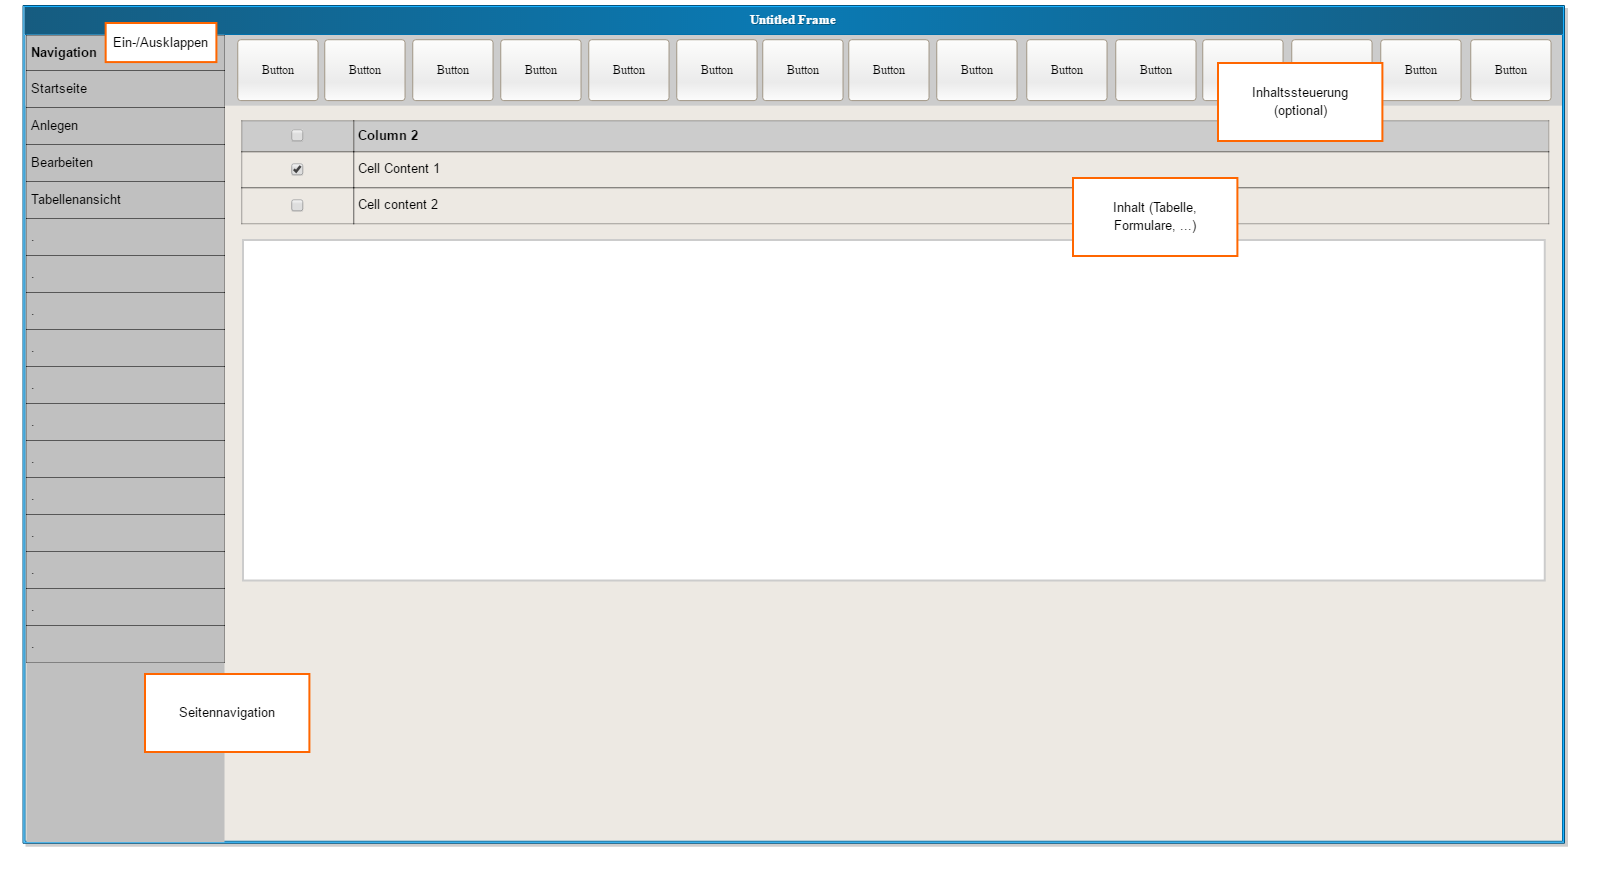
\includegraphics[width=1\textwidth]{mockupaufteilung.png}
	\captionof{figure}{Seitenaufbau}
	\label{Seitenaufbau}
\end{minipage}

\pagebreak
\eject

\section{Planung}
Laut ECTS (8) -> SWS (ca. 5) ergibt sich eine Investition von ca. 70 Arbeitsstunden.

\section{Umsetzung}
Agile Entwicklung während des Projekts (angelehnt an Scrum):
\begin{enumerate}
	\item Wählen eines Projektpakets (Funktionale Anforderungen)
	\item Definition des Ziels
	\item Implementierung
	\item Testing
	\item Abschluss des Blocks
\end{enumerate}

\subsection{Zeitplanung}
\begin{tabularx}{\textwidth}{|l|X|l|l|}
	\hline
	Nr. & Inhalt & Frist & Erledigt \\ \hline
	1 & Vorbesprechung Projektbetreuer & 11. September 2018 & 11. September 2018 \\ \hline
	2 & Vorbesprechung LVMWNRW & 15. September 2018 & 15. September 2018 \\ \hline
	3 & Kickoff Repository & 01. Oktober 2018 & 18. September 2018 \\ \hline
	4 & Offizieller Projektstart & 08. Oktober 2018 & 08. Oktober 2018 \\ \hline
	5 & Ende Phase 1 & 01. November 2018 & ??? \\ \hline
	6 & Ende Phase 2a & 01. Dezember 2018 & ??? \\ \hline
	7 & Ende Phase 2b & 07. Dezember 2018 & ??? \\ \hline
	8 & Testlauf 1 & 07. Dezember 2018 & ??? \\ \hline
	9 & Besprechung LVMWNRW & 08. Dezember 2018 & ??? \\ \hline
	10 & Ende Phase 3 & 31. Januar 2019 & ??? \\ \hline
	11 & Projektbereinigung & 07. Februar 2019 & ??? \\ \hline
	12 & Abgabe & 08. Februar 2019 & ??? \\ \hline
\end{tabularx}

\subsection{Phasen}
\subsubsection{Phase 0}
	Erlernen der Grundlagen und aufsetzen der Entwicklungsumgebung.
	
	\begin{itemize}
		\item Typescript
		\item Angular
		\item Electron
		\item Nebular
	\end{itemize}

\subsubsection{Phase 1}
	\begin{itemize}
		\item Konzept:
		\item Umsetzung:
		\item Testläufe:
	\end{itemize}
	
\subsubsection{Phase 2}
	\begin{itemize}
		\item Konzept:
		\item Umsetzung:
		\item Testläufe:
	\end{itemize}

\subsubsection{Phase 3}
	\begin{itemize}
		\item Konzept:
		\item Umsetzung:
		\item Testläufe:
	\end{itemize}

\subsubsection{Resümee}
	\begin{itemize}
		\item Status quo:
		\item Testdurchlauf:
		\item Fazit (''What we have learned''):
		\item Abschlussbericht:
		\item Präsentation:
		\item Studienprojektbewertung:
	\end{itemize}


\pagebreak
\eject

\section{Erweiterungen}
Für ein Projekt dürften die Bausteine aus dem letzten Kapitel bereits mehr als ausreichend sein. Trotzdem soll an dieser Stelle kurz weiter geträumt werden:

\begin{itemize}
	\item Daten generieren: Automatische Zimmerbelegung, Stundenplan, ...
	\item Website mit Zugriff für Teilnehmer
	\item Bewerbung via Website
	\item Verwaltungs-App
	\item Rahmenprogrammplaner: Alle können etwas posten, dies wird dann verteilt
	\item ...
\end{itemize}
	
\pagebreak
\eject
	
\end{document}
